\documentclass[12pt,a4paper]{article}
\usepackage[utf8]{vietnam}
\usepackage{amsmath,amssymb}
\usepackage{tabularx}
\usepackage{tikz}
\usetikzlibrary{calc,angles,quotes,arrows.meta,patterns}
\usepackage{xcolor}
\usepackage{enumitem}
\usepackage{fancyhdr}
\usepackage[top=1.2cm, bottom=1.2cm, left=1.5cm, right=1.5cm]{geometry}
\usepackage[dethi]{ex_test}
\SAOPTN{widthSA=2.6,heightSA=0.62}

\setlength{\headheight}{15pt}
\setlength{\parskip}{0pt}

\pagestyle{fancy}
\fancyhf{}
\rhead{\textit{Môn Toán 6 -- Đề số 6}}
\lhead{\textit{Bộ đề ôn tập Giữa học kì I}}
\cfoot{\thepage}

\begin{document}

% --- KHUNG TIÊU ĐỀ ĐỀ THI ---
\noindent
\begin{tabularx}{\linewidth}{X r}
\textbf{TRƯỜNG THCS: \dotfill} & \textbf{ĐỀ KIỂM TRA ĐỊNH KỲ GIỮA HỌC KỲ I} \\
\textbf{Họ và tên: \dotfill} & \textbf{NĂM HỌC 2026 -- 2027} \\
\textbf{Lớp: \dotfill \quad SBD: \dotfill} & \textbf{Môn: TOÁN 6} \\
\hline
\end{tabularx}
\vspace{2mm}

\begin{center}
  \textbf{\large ĐỀ ÔN TẬP GIỮA HỌC KỲ I -- ĐỀ SỐ 6}\\
  \textit{Thời gian làm bài: 90 phút (Không kể thời gian phát đề)}
\end{center}
\vspace{1mm}

% --- PHẦN I ---
\noindent\textbf{\large PHẦN I. CÂU TRẮC NGHIỆM NHIỀU PHƯƠNG ÁN LỰA CHỌN (3,0 điểm)}

\textit{Thí sinh trả lời từ câu 1 đến câu 12. Mỗi câu hỏi thí sinh chỉ chọn một phương án duy nhất.}

\vspace{1mm}
\begin{ex}
Khẳng định nào sau đây là sai?\\Trong hình vuông:
\choice
{Bốn cạnh bằng nhau}
{\True Hai đường chéo song song với nhau}
{Bốn góc ở các đỉnh là góc vuông}
{Hai cạnh đối song song}
\end{ex}

\begin{ex}
Cho tập hợp $A = \{0; 2; 4; a; b\}$. Khẳng định nào dưới đây sai?
\choice
{\True $5 \in A$}
{$a \in A$}
{$0 \in A$}
{$1 \notin A$}
\end{ex}

\begin{ex}
Cho tập hợp $A = \{x \in \mathbb{N}^* \mid x \le 4\}$. Số nào dưới đây là phần tử của $A$?
\choice
{0}
{\True 4}
{5}
{6}
\end{ex}

\begin{ex}
Với $a, m, n$ là các số tự nhiên, khẳng định nào sau đây đúng?
\choice
{\True $a^m : a^n = a^{m-n}$ ($a \ne 0, m \ge n$)}
{$a^m : a^n = a^{m+n}$ ($a \ne 0$)}
{$a^m : a^n = a^{m \cdot n}$ ($a \ne 0$)}
{$a^m : a^n = m - n$ ($a \ne 0$)}
\end{ex}

\begin{ex}
Kết quả của phép tính $256 - 98 + 137$ là:
\choice
{21}
{217}
{259}
{\True 295}
\end{ex}

\begin{ex}
Đối với biểu thức không có dấu ngoặc và chỉ có các phép tính cộng, trừ, nhân, chia, lũy thừa, thì thứ tự thực hiện phép tính đúng là:
\choice
{Nhân và chia $\to$ Lũy thừa $\to$ Cộng và trừ}
{\True Lũy thừa $\to$ Nhân và chia $\to$ Cộng và trừ}
{Lũy thừa $\to$ Cộng và trừ $\to$ Nhân và chia}
{Cộng và trừ $\to$ Nhân và chia $\to$ Lũy thừa}
\end{ex}

\begin{ex}
Cho các số $3; 15; 29$. Số không là số nguyên tố trong các số đó là:
\choice
{3}
{\True 15}
{29}
{Cả 3 số trên}
\end{ex}

\begin{ex}
Trong các số sau, số nào chia hết cho 9?
\choice
{\True 144}
{249}
{379}
{199}
\end{ex}

\begin{ex}
Bạn An có ngày sinh là số nguyên tố lớn nhất nhỏ hơn 20, tháng sinh của bạn là số nguyên tố nhỏ nhất. Vậy bạn An có ngày và tháng sinh là:
\choice
{Ngày 19 tháng 3}
{\True Ngày 19 tháng 2}
{Ngày 7 tháng 2}
{Ngày 7 tháng 3}
\end{ex}

\begin{ex}
Hình nào dưới đây là tam giác đều?
\begin{center}
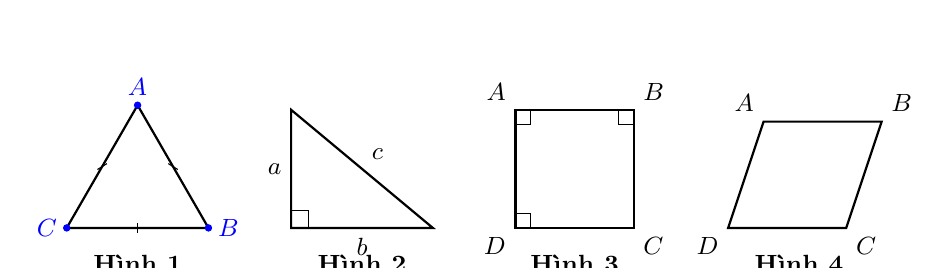
\begin{tikzpicture}[scale=0.75, font=\small]
  % Hinh 1: Tam giac deu ABC
  \begin{scope}[shift={(0,0)}]
    \coordinate (C) at (0,0);
    \coordinate (B) at (2.4,0);
    \coordinate (A) at (1.2, 2.078);
    \draw[thick] (A) -- (B) -- (C) -- cycle;
    \filldraw[blue] (A) circle (1.5pt) node[above] {$A$};
    \filldraw[blue] (B) circle (1.5pt) node[right] {$B$};
    \filldraw[blue] (C) circle (1.5pt) node[left] {$C$};
    \draw ($(A)!0.5!(B) + (-0.08,0.05)$) -- ($(A)!0.5!(B) + (0.08,-0.05)$);
    \draw ($(A)!0.5!(C) + (-0.08,-0.05)$) -- ($(A)!0.5!(C) + (0.08,0.05)$);
    \draw ($(B)!0.5!(C) + (0,-0.09)$) -- ($(B)!0.5!(C) + (0,0.09)$);
    \node at (1.2, -0.6) {\textbf{Hình 1}};
  \end{scope}
  % Hinh 2: Tam giac vuong
  \begin{scope}[shift={(3.8,0)}]
    \coordinate (V) at (0,0);
    \coordinate (X) at (2.4,0);
    \coordinate (Y) at (0,2);
    \draw[thick] (V) -- (X) -- (Y) -- cycle;
    \draw (0,0.3) -- (0.3,0.3) -- (0.3,0);
    \node[left] at (0,1) {$a$};
    \node[below] at (1.2,0) {$b$};
    \node[above right] at (1.2,1) {$c$};
    \node at (1.2, -0.6) {\textbf{Hình 2}};
  \end{scope}
  % Hinh 3: Hinh vuong ABCD
  \begin{scope}[shift={(7.6,0)}]
    \coordinate (D) at (0,0);
    \coordinate (C3) at (2,0);
    \coordinate (B3) at (2,2);
    \coordinate (A3) at (0,2);
    \draw[thick] (A3) -- (B3) -- (C3) -- (D) -- cycle;
    \draw (0,1.75) -- (0.25,1.75) -- (0.25,2);
    \draw (2,1.75) -- (1.75,1.75) -- (1.75,2);
    \draw (0,0.25) -- (0.25,0.25) -- (0.25,0);
    \node[above left] at (A3) {$A$};
    \node[above right] at (B3) {$B$};
    \node[below right] at (C3) {$C$};
    \node[below left] at (D) {$D$};
    \node at (1, -0.6) {\textbf{Hình 3}};
  \end{scope}
  % Hinh 4: Hinh binh hanh ABCD
  \begin{scope}[shift={(11.2,0)}]
    \coordinate (D4) at (0,0);
    \coordinate (C4) at (2,0);
    \coordinate (B4) at (2.6,1.8);
    \coordinate (A4) at (0.6,1.8);
    \draw[thick] (A4) -- (B4) -- (C4) -- (D4) -- cycle;
    \node[above left] at (A4) {$A$};
    \node[above right] at (B4) {$B$};
    \node[below right] at (C4) {$C$};
    \node[below left] at (D4) {$D$};
    \node at (1.2, -0.6) {\textbf{Hình 4}};
  \end{scope}
\end{tikzpicture}
\end{center}
\choice
{\True Hình 1}
{Hình 2}
{Hình 3}
{Hình 4}
\end{ex}

\begin{ex}
Mỗi góc của lục giác đều có số đo bằng:
\choice
{$90^\circ$}
{$180^\circ$}
{\True $120^\circ$}
{$60^\circ$}
\end{ex}

\begin{ex}
Một mảnh giấy hình chữ nhật có diện tích $120\text{ cm}^2$, độ dài một cạnh là $8\text{ cm}$. Chu vi của mảnh giấy là:
\choice
{$34\text{ cm}$}
{$40\text{ cm}$}
{\True $46\text{ cm}$}
{$54\text{ cm}$}
\end{ex}


\vspace{1mm}
\noindent\textbf{BẢNG TRẢ LỜI TRẮC NGHIỆM PHẦN I:}
\begin{center}
\begin{tabular}{|c|c|c|c|c|c|c|c|c|c|c|c|c|}
\hline
\textbf{Câu} & \textbf{1} & \textbf{2} & \textbf{3} & \textbf{4} & \textbf{5} & \textbf{6} & \textbf{7} & \textbf{8} & \textbf{9} & \textbf{10} & \textbf{11} & \textbf{12} \\
\hline
\textbf{Chọn} & \rule{0pt}{0.65cm} & & & & & & & & & & & \\
\hline
\end{tabular}
\end{center}
\vspace{2mm}

\setcounter{ex}{0}
\noindent\textbf{\large PHẦN II. CÂU TRẮC NGHIỆM ĐÚNG SAI (2,0 điểm)}

\textit{Thí sinh trả lời câu 1 và câu 2. Trong mỗi ý a), b), c), d) ở mỗi câu, thí sinh chọn đúng hoặc sai.}

\vspace{1mm}
\begin{ex}
Cho hình vuông $ABCD$ có cạnh bằng $4\text{ cm}$. Xét tính đúng/sai của các khẳng định sau:
\choiceTF
{\True $AB = BC = CD = DA = 4\text{ cm}$}
{$AB$ và $BD$ song song với nhau}
{Mỗi góc ở các đỉnh của hình vuông bằng nhau và bằng $60^\circ$}
{\True Vẽ cạnh $AB = 4\text{ cm}$. Dùng thước êke vẽ các đường vuông góc với $AB$ tại $A$ và $B$, sau đó lần lượt lấy các điểm $D, C$ trên các đường đó sao cho $AD = BC = 4\text{ cm}$. Nối $C$ với $D$ ta được hình vuông $ABCD$ có cạnh $4\text{ cm}$ như đã cho}
\end{ex}

\begin{ex}
Cho tập hợp $A = \{x \in \mathbb{N} \mid 10 < x \le 15\}$. Xét tính đúng/sai của các khẳng định sau:
\choiceTF
{\True Tập hợp $A$ được viết dưới dạng liệt kê các phần tử là: $A = \{11; 12; 13; 14; 15\}$}
{Số 10 thuộc tập hợp $A$ (kí hiệu là $10 \in A$)}
{\True Trong tập hợp $A$, có đúng 2 phần tử là số nguyên tố}
{Tổng của phần tử lớn nhất và phần tử bé nhất trong tập hợp $A$ là một số chia hết cho 3}
\end{ex}


\noindent\textbf{BẢNG TRẢ LỜI PHẦN II:}
\begin{center}
\begin{tabular}{|c|c|c|c|c||c|c|c|c|c|}
\hline
\textbf{Câu 1} & \textbf{a)} & \textbf{b)} & \textbf{c)} & \textbf{d)} & \textbf{Câu 2} & \textbf{a)} & \textbf{b)} & \textbf{c)} & \textbf{d)} \\
\hline
\textbf{Đ/S} & \rule{0pt}{0.6cm} & & & & \textbf{Đ/S} & & & & \\
\hline
\end{tabular}
\end{center}
\vspace{2mm}

\setcounter{ex}{0}
\noindent\textbf{\large PHẦN III. CÂU HỎI TRẢ LỜI NGẮN (2,0 điểm)}

\textit{Thí sinh trả lời câu 1 và câu 2. Điền kết quả số vào ô trống tương ứng.}

\vspace{1mm}
\begin{ex}
Tìm số tự nhiên $x$ thỏa mãn $2^x \cdot 4 = 32$. \shortans{3}
\end{ex}

\begin{ex}
Một hình chữ nhật có chu vi bằng $28\text{ cm}$ và chiều dài bằng $8\text{ cm}$. Tính diện tích của hình chữ nhật đó (theo đơn vị $\text{cm}^2$). \shortans{48}
\end{ex}


\setcounter{ex}{0}
\noindent\textbf{\large PHẦN IV. TỰ LUẬN (3,0 điểm)}

\textit{Thí sinh trình bày chi tiết lời giải vào giấy làm bài.}

\vspace{1mm}
\begin{ex} (1,5 điểm)
Thực hiện phép tính (Tính hợp lí nếu có thể):
\begin{enumerate}[label=\textbf{\alph*)}, leftmargin=0.8cm, itemsep=2pt]
\item (0,5 điểm) $12 \cdot 25 + 85 : 17 - 205$
\item (0,5 điểm) $5^2 \cdot 13 - 5^2 \cdot 3$
\item (0,5 điểm) $57 - [250 : (7 - 2)^2 - 3] \cdot 2025^0$
\end{enumerate}
\end{ex}
\vspace{1.5mm}

\begin{ex} (1,5 điểm)
Tìm số tự nhiên $x$, biết:
\begin{enumerate}[label=\textbf{\alph*)}, leftmargin=0.8cm, itemsep=2pt]
\item (0,5 điểm) $x + 12 = 45$
\item (0,5 điểm) $333 - x = 5^6 : 5^3$
\item (0,5 điểm) $(2x + 2)^3 = 12 \cdot 144$
\end{enumerate}
\end{ex}
\vspace{1.5mm}

\begin{ex} (1,5 điểm)
Kích thước chuẩn của sân bóng đá mini cho 5 người là sân hình chữ nhật có chiều dài tối thiểu $25\text{ m}$ và tối đa $42\text{ m}$, chiều rộng tối thiểu $15\text{ m}$ và tối đa $25\text{ m}$. Trường THCS A xây dựng sân bóng đá cỏ nhân tạo hình chữ nhật có chiều dài $30\text{ m}$, chiều rộng $20\text{ m}$.
\begin{enumerate}[label=\textbf{\alph*)}, leftmargin=0.8cm, itemsep=2pt]
\item (0,75 điểm) Vẽ minh họa sân bóng đá hình chữ nhật $ABCD$ có cạnh $AB = 3\text{ cm}$ và cạnh $BC = 2\text{ cm}$.
\item (0,75 điểm) Tính diện tích sân bóng đó.
\end{enumerate}
\end{ex}
\vspace{1.5mm}

\begin{ex} (0,5 điểm)
Một người bán 6 giỏ cam và xoài. Mỗi giỏ chỉ đựng hoặc cam hoặc xoài với số lượng sau: 34 quả, 39 quả, 40 quả, 41 quả, 42 quả, 46 quả. Sau khi bán một giỏ xoài thì số cam còn lại gấp 4 lần số xoài còn lại. Hãy cho biết giỏ nào đựng cam, giỏ nào đựng xoài?
\end{ex}
\vspace{1.5mm}


\begin{center}
\rule{4cm}{0.4pt}\\
\textit{--- HẾT ---}
\end{center}
\end{document}
